\documentclass[12pt,a4paper]{article}
\usepackage{times}
\usepackage{appendix}
\usepackage{mathptmx}
\usepackage{setspace}
\usepackage[utf8]{inputenc}
\usepackage[french]{babel}
\usepackage[T1]{fontenc}
\usepackage{amsmath}
\usepackage{amsfonts}
\usepackage{amssymb}
\usepackage{makeidx}
\usepackage{graphicx}
\usepackage{lmodern}
\usepackage{index}
\usepackage{diagbox}
\usepackage{multirow}
\newcommand{\HRule}{\rule{\linewidth}{0.5mm}}
\usepackage{fourier}
\usepackage[left=2cm,right=2.5cm,top=2.5cm,bottom=2.5cm]{geometry}
\author{Sarah Kaddah}
\title{Rapport de stage}
%%%%%%%%%%Interligne%%%%%%%%%%
\renewcommand{\baselinestretch}{1.5}
\begin{document}
%%%%%%%%%%%%%%%%%%%%%%%%%%%%%%%%%%%%%%%%%%%%%%%%%%%%%%%%%%%%%%%%%
%%%%%%%%%%%%%%%%%%%%%%1ere page%%%%%%%%%%%%%%%%%%%%%%%%%%%%%%%%%%
%%%%%%%%%%%%%%%%%%%%%%%%%%%%%%%%%%%%%%%%%%%%%%%%%%%%%%%%%%%%%%%%%
%%%%%%%%%%%%%%%%%%%%%%%%%%%%%%%%%%%%%%%%%%%%%%%%%%%%%%%%%%%%%%%%%
%%%%%%%%% Header %%%%%%%%%
	\begin{titlepage}
	\begin{sffamily}
	\begin{center}
	\large{Université Paris Diderot - Paris 7 \hfill 2017-2018} \bigskip
	\center{\LARGE{Master 2 Biologie-Informatique/ Bioinformatique}}	
	\begin{tabular}{c}
		\\ \\ \\
		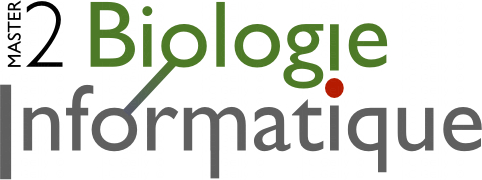
\includegraphics[scale=0.3]{img/m2.png}
	\end{tabular}
	\hfill
	\begin{tabular}{c}
		\\
		
\includegraphics[scale=0.1]{img/p7.png}
	\end{tabular}
%%%%%%%%% Title %%%%%%%%%
    \HRule \\[0.2cm]
    { \huge \bfseries \center{Classification pour l'étude des séquences répétées centromériques chez les primates}\\[0.4cm]}
    \HRule \\%[2cm]
%%%%%%%% Center %%%%%%%%
\begin{center}\LARGE{\textbf{Sarah Kaddah}}\end{center}
%%%%%%%%% Footer %%%%%%%%%
\begin{center}\Large{Tuteur: Lo\"{i}c Ponger}\end{center}~\\
\center{\large{Structure et Instabilité des Génomes}}
\center{\large{ MNHN - CNRS UMR 7196 / INSERM U1154 - Sorbonne Universités}}\\
Muséum national d'Histoire naturelle, 43 rue Cuvier 75005 PARIS \\ [1cm]
%%%%%%%%% Logos %%%%%%%%%
\begin{tabular}{cc}
	\hspace*{2.5cm} &  
	
\includegraphics[scale=0.2]{img/mnhn.jpg}
\end{tabular}
	\hfill
\begin{tabular}{c}
	
\includegraphics[scale=0.08]{img/inserm.jpg}
\end{tabular}
	\hfill
\begin{tabular}{cc}
	
\includegraphics[scale=0.08]{img/cnrs.png} &
	\hspace*{2.5cm}
\end{tabular}
	\end{center}
	\end{sffamily}
\end{titlepage}

%%%%%%%%%%%%%%%%%%%%%%%%%%%%%%%%%%%%%%%%%%%%%%%%%%%%%%%%%%%%%%%%%%
%%%%%%%%%%%%%%%%%%%%%Remerciements%%%%%%%%%%%%%%%%%%%%%%%%%%%%%%%%
%%%%%%%%%%%%%%%%%%%%%%%%%%%%%%%%%%%%%%%%%%%%%%%%%%%%%%%%%%%%%%%%%%
\section*{\begin{center}Remerciements\end{center}}~\\[0.2cm]
\addcontentsline{toc}{section}{Remerciements}
Je tiens tout d’abord à remercier énormément Loïc Ponger, responsable de mon stage, pour
son encadrement, ses conseils, ses relectures et son aide.\\

Je tiens également à remercier Christophe Escudé pour tous ses conseils et pour la
relecture de mon rapport, ainsi que l'équipe ARChE.\\

Je souhaite aussi remercier Evelyne Duvernois-Berthet, pour ses conseils tant au niveau professionnel
que personnel, pour les discussions et pour les bonbons.\\

Je remercie aussi chaleureusement tout le laboratoire pour son accueil cordial.\\

Je remercie le journal club pour ces petites séances d'anglais sympathiques.\\

Je souhaite également remercier ici Catherine Etchebest et Jean-Christophe Gelly, et l’en-
semble de l’équipe pédagogique, pour cette année de master 2.\\

\thispagestyle{empty}

%%%%%%%%%%%%%%%%%%%%%%%%%%%%%%%%%%%%%%%%%%%%%%%%%%%%%%%%%%%%%%%%%%
%%%%%%%%%%%%%%%%%%%Table des matières%%%%%%%%%%%%%%%%%%%%%%%%%%%%
%%%%%%%%%%%%%%%%%%%%%%%%%%%%%%%%%%%%%%%%%%%%%%%%%%%%%%%%%%%%%%%%%
\newpage
\tableofcontents
\setcounter{page}{0}
\thispagestyle{empty}
\newpage 

%%%%%%%%%%%%%%%%%%%%%%%%%%%%%%%%%%%%%%%%%%%%%%%%%%%%%%%%%%%%%%%%
%%%%%%%%%%%%%%%%%%%%Introduction%%%%%%%%%%%%%%%%%%%%%%%%%%%%%%%%
%%%%%%%%%%%%%%%%%%%%%%%%%%%%%%%%%%%%%%%%%%%%%%%%%%%%%%%%%%%%%%%% 
\section{Introduction}
\subsection{Le centromère}
Le centromère est une structure chromatinienne essentielle au bon déroulement de la division cellulaire chez les eucaryotes. Il permet l'attachement du fuseau mitotique et la ségrégation des chromosomes \cite{Cleveland2003}.  Le kinétochore est un assemblage de protéines situé au niveau du centromère.  Il va permettre l'attachement des  microtubules aux chromosomes \cite{Santaguida2009}. La chromatine centromérique est caractérisée par la présence de la protéine CENP-A, un variant de l'histone H3, très conservé au cours de l'évolution. Celle-ci fixe la position du kinetochore par un mécanisme épigénétique encore mal connu \cite{Sullivan1994}.

Bien que la fonction du centromère et des protéines sous-jacentes soit relativement bien conservée, les séquences d'ADN associées varient d'un taxon à l'autre. Cependant une structure commune se distingue étant de l'ADN répété en tandem, appelée ADN satellite \cite{Henikoff2001}. Ces séquences peuvent représenter environ 5\% du génome et la taille des unités de répétitions peut varier entre 7pb et 3,2kb \cite{Cellamare2009}.

\subsection{L'ADN $\alpha$-satellite}
Chez les Primates, l'ADN satellite le plus abondant est connu sous le nom d'$\alpha$-satellite. Ces séquences sont riches en AT et un monomère fait 171 pb de long environ \cite{Willard1991}. Ces séquences ont été mises en évidence pour la première fois chez \textit{Chlorocebus aethiops} dans les années 1970 \cite{Kurnit1974}. Des homologues ont été retrouvés chez d’autres espèces de primates \cite{Lee1997}. Néanmoins, ces séquences ont été essentiellement étudiées chez l’Homme.

Les séquences ont un taux d’identité qui varie de  60 à 100\% \cite{Alexandrov2001}. Les séquences les plus similaires peuvent être regroupées en familles (Figure \ref{shepelev}). Ces familles résultent d'un même événement d'amplification. Des études chez l'Homme ont montré que les séquences d'une même famille se regroupent phylogénétiquement mais aussi spatialement le long d'un chromosome \cite{Shepelev2009}. Les familles se disposent de façon symétrique autour du cœur du centromère en respectant un gradient d'âge.  Ces observations ont permis de proposer un modèle évolutif avec des centromères en expansion. Les familles les plus récentes s’inséreraient au cœur du centromère, dans la partie active, repoussant les familles les plus anciennes jusqu'aux régions voisines, appelées péri-centromères. Les familles les plus anciennes ont une organisation monomérique, sous forme de longs segments composés de monomères de la même famille. Les familles récentes sont organisées en structure d'ordre supérieur ou \textit{Higher Order Repeat} (HOR), où un groupe de monomères appartenant à des familles différentes est répété en bloc en tandem ( Figure \ref{organisation_spatiale}).

\begin{figure}
	\center
		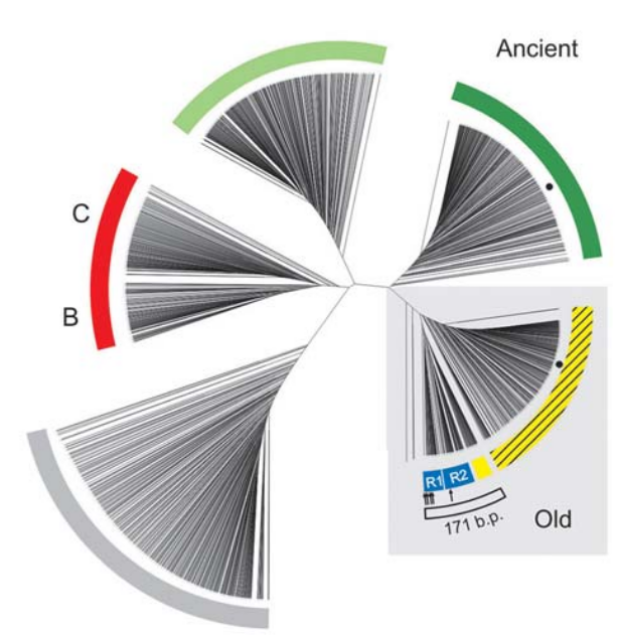
\includegraphics[height=6cm, width=6cm]{img/shepelev.png}
		\caption{\textbf{Arbre phylogénétique des séquences $\alpha$-satellites du bras p du chromosome X chez l'Homme:} L’arbre réunit 1431 monomères présents sur le contig nt011630 \cite{Shepelev2009}.\label{shepelev}}
\end{figure}

Le rôle des $\alpha$-satellites est encore mal connu dans la fonction du centromère, mais des études chez l'Homme ont permis de mettre en évidence l'existence des motifs CENP-B et pJ$\alpha$. Ces deux motifs seraient capable de lier respectivement les protéines CENP-B et pJ$\alpha$, cette dernière étant très mal caractérisée. Un troisième motif pK$\beta$ a récemment été mis en évidence par l'équipe. Ces trois motifs sont exclusifs l'un de l'autre et se situent au même endroit sur une séquence. La fonction de ces trois motifs est encore inconnue.

\begin{figure}
\center
	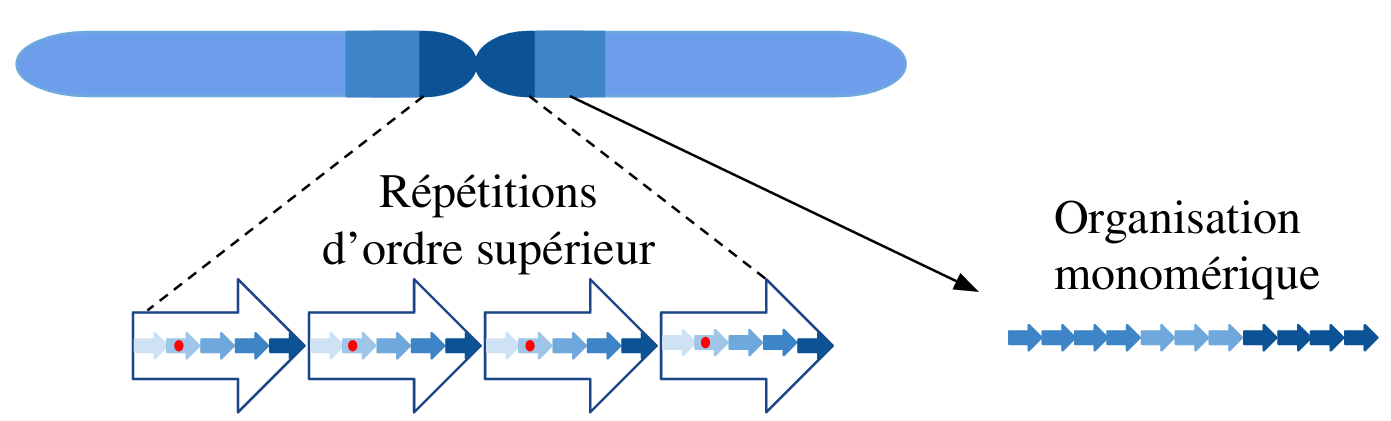
\includegraphics[height=3.5cm, width=12cm]{img/AS_organization.png}
	\caption{\textbf{Organisation spatiale des $\alpha$-satellites:} Le cœur du centromère (bleu foncé) est organisé en répétitions d'ordre supérieur. Le péricentromère (bleu clair) a une organisation monomérique. Les monomères sont représentés par une flèche bleue. Les flèches d'une même nuance de couleur appartiennent à la même famille. Les points rouges représentent les motifs CENP-B, pJ$\alpha$ ou pK$\beta$. \label{organisation_spatiale}}
\end{figure}

\subsection{Le sujet de stage}

L'objectif de ce stage est d'étudier les $\alpha$-satellites à partir de données de séquençage haut débit afin de mieux comprendre la fonction  et les mécanismes d'évolution de ces séquences. 

Peu d'informations sur les $\alpha$-satellites existent chez les espèces de primates. De plus, aucune relation inter-espèce n'a été réalisée, le séquençage et l'assemblage de ces séquences étant difficiles de par leur caractère répété. Jusqu'à présent, les études se basant sur un séquençage haut-débit ont été appliquées chez l'Homme (cité ci-dessus) et chez le Gorille. L'équipe d'accueil de mon stage "ADN répété, Chromatine, Evolution" ou ARChE, a récemment développé une approche de séquençage haut débit, ciblée sur les séquences $\alpha$-satellites chez \textit{Cercopithecus solatus} \cite{Cacheux2016} et \textit{Cercopithecus pogonias} \cite{Cacheux2018}. Ces deux espèces ont été choisies car elles présentent beaucoup d'ADN satellite et de réarrangements chromosomiques, avec l'apparition de nombreux centromères. Cette étude a montré les limites des approches classiques (alignements et phylogénie) car elles ne permettent pas de traiter des jeux de données de grande taille. Or il peut y avoir plusieurs milliers de  monomères dans un seul génome. De plus, elles ne permettent pas de faire des comparaisons entre espèces.

Pour remédier à ce problème, une méthode de classification automatisée des $\alpha$-satellites a été développée dans l'équipe (Jornod, Master 2 2016-2017). Elle permet de traiter des centaines de milliers de séquences, quelque soit le nombre ou la taille des familles. De plus, cette méthode est objective et peut être appliquée à plusieurs espèces, permettant ainsi une comparaison inter-espèce des familles $\alpha$-satellites. 

Afin d'évaluer cette méthode, je  vais l'appliquer aux jeux de données déjà publiés. Dans un second temps, cette méthode est appliquée à deux autres primates dans le but de  caractériser les familles d'espèces proches. Les mécanismes d'évolution pourront être déduits à partir d'une comparaison inter-espèce révélant les différences et les familles communes.

%%%%%%%%%%%%%%%%%%%%%%%%%%%%%%%%%%%%%%%%%%%%%%%%%%%%%%%%%%%%%%%%%
%%%%%%%%%%%%%%%%%%%%%%M & M%%%%%%%%%%%%%%%%%%%%%%%%%%%%%%%%%%%%%%
%%%%%%%%%%%%%%%%%%%%%%%%%%%%%%%%%%%%%%%%%%%%%%%%%%%%%%%%%%%%%%%%% 
\section{Matériel et méthode}
\subsection{Les espèces étudiées}

	\begin{figure}
		\center
		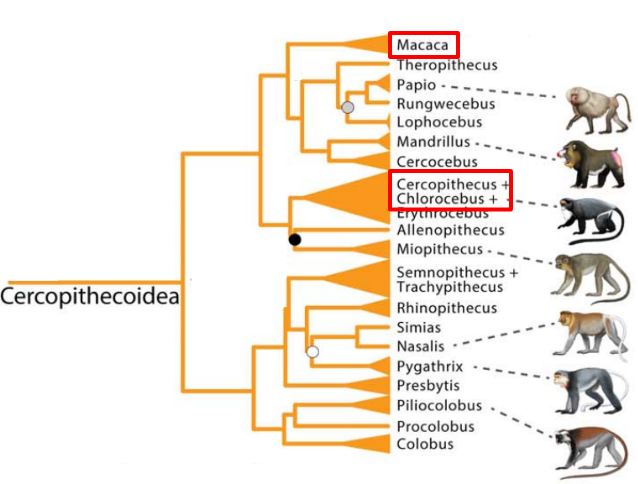
\includegraphics[height=6.5cm, width=9cm]{img/arbre_presentation.png}
		\caption{\textbf{Arbre phylogénétique des espèces analysées.}\cite{Springer2012}
		\label{fig:arbre_presentation}}
	\end{figure}

Les deux espèces \textit{C. solatus} et \textit{C. pogonias}, dont les jeux de données sont déjà publiés, sont d'abord choisies. Ces données sont issues d'un séquençage ciblé de monomères digérés par une enzyme de restriction (XmnI, HindIII) et séquencés en Ion Torrent \cite{Benjak2015}. 

Ensuite, une recherche d'$\alpha$-satellites chez d'autres primates, issus du séquençage à haut débit, a été réalisée sur Genbank. Afin de permettre de comparer les données avec les deux Cercopithèques, j'ai choisi deux espèces proches parmi 10 espèces selon la disponibilité des données et la qualité des séquences (Figure \ref{fig:arbre_presentation}), \textit{Macaca fascicularis} et \textit{Chlorocebus sabaeus}.

Les monomères d'$\alpha$-satellites faisant environ 171pb,  seuls les projets impliquant des reads relativement longs ont été considérés (Illumina en single-end, L454, ...). Tous les $\alpha$-satellites sont alignés (même phase) sur les monomères de \textit{C. solatus} et \textit{C. pogonias} étudiés précédemment.


\subsection{Méthode de classification}
	\subsubsection{Principe}
Cette méthode a été développée par Florence Jornod (stage M2, 2016-2017). Elle répartit des séquences $\alpha$-satellites en familles selon la similarité calculée à partir de leur composition en 5-mers. La classification est hiérarchique dichotomique. Au départ, une table contenant les fréquences des 5-mers est calculée pour chaque monomère. Ensuite une boucle itérative est exécutée pour séparer les séquences en deux groupes (voir 2.2.2). Cette étape est répétée tant que les nouveaux groupes formés sont divisibles (schéma de l'algorithme en annexe).

	\subsubsection{Répartition itérative}
Une Analyse en Composante Principale (ACP) est effectuée sur la table des fréquences des 5-mers afin de réduire les dimensions du jeu de données et d’obtenir des variables indépendantes. Les distances euclidiennes sont calculées entre toutes les paires de séquences dans l’espace défini par 1024 composantes de l’ACP. 

A partir du calcul de distance, les séquences sont séparées en deux classes en utilisant la classification hiérarchique basée sur la méthode de Ward. Cette méthode maximise l’inertie interclasse. La classification hiérarchique fait un usage important de la mémoire. Par conséquent, pour traiter des jeux de données importants, la classification est appliquée à 100 000 séquences choisies aléatoirement et une analyse discriminante linéaire (LDA) est utilisée pour classer les autres séquences.

	\subsubsection{Double-validation d'un sous-groupe}
A chaque itération, la classification hiérarchique divise le jeu de données en deux groupes qui sont évalués avant d'être ou non redivisés. Afin d'éviter de diviser les données en familles trop petites, le premier critère de validation est la taille du sous-groupe. Si un groupe fait moins de 100 séquences, il n'est pas redivisé. Le deuxième critère de validation s'appuie sur le \textit{matepair} et permet d'estimer la qualité de la partition. Ce terme correspond à la proportion de monomères ayant son plus proche voisin dans la même classe, se basant sur les distances euclidiennes calculées auparavant. Ainsi des valeurs de \textit{matepairs} élevées (proches de 1) indiquent des sous-groupes bien homogènes et séparés validant la classification.

Le seuil de \textit{matepair} est fixé à 0.90, pour avoir des groupes homogènes. Si au moins une des valeurs de \textit{matepair} est au-dessous de ce seuil, les sous-groupes sont considérés comme formant un seul groupe et le groupe initial est sauvegardé comme une famille unique. Si les \textit{matepairs} sont au-dessus d’un certain seuil, les deux sous-groupes sont ajoutés séparément à la file pour être potentiellement redivisés ultérieurement.

	\subsection{Analyse des séquences}
	
Les séquences monomériques sont comparées à partir de leur composition en 5-mers dans le but d'identifier des regroupements d'$\alpha$-satellites sans passer par l'étape d'alignement. Pour chaque ensemble de monomères,	la table de fréquence des 5-mers est analysée en utilisant l'Analyse en Composante Principale (ACP) pour réduire l'espace de complexité pour pourvoir visualiser les données sur les premiers plans factoriels.
	
L'alignement des séquences est fait avec Muscle \cite{Edgar2004} et visualisé avec Seaview \cite{Galtier1996}. La phylogénie est construite avec la méthode du maximum de vraisemblance (PhyML) \cite{Guindon2009}. Le modèle F84 est utilisé pour la construction de l'arbre. Le support de branche est aLRT (SH-like). La fréquence d'équilibre des nucléotides, le ratio de transition et de transversion et les taux de variation sont optimisés.

Les consensus sont obtenus avec des scripts développés par l'équipe. Les motifs CENP-B (TTCGTTGGAA[AG]CGGGA), PJ$\alpha$ (TTCCTTTT[CT]CACC[AG]TAG) et pK$\beta$ (GATATCCCGGTTTCCTT) ont été identifiés avec le logiciel fuzznuc (package EMBOSS) \cite{Rice2000} et en autorisant 2 \textit{mismatch} au maximum par rapport au consensus.

%%%%%%%%%%%%%%%%%%%%%%%%%%%%%%%%%%%%%%%%%%%%%%%%%%%%%%%%%%%%%%%%%
%%%%%%%%%%%%%%%%%%%%%%Résultats 1%%%%%%%%%%%%%%%%%%%%%%%%%%%%%%%%
%%%%%%%%%%%%%%%%%%%%%%%%%%%%%%%%%%%%%%%%%%%%%%%%%%%%%%%%%%%%%%%%% 
\section{Résultats}
	\subsection{Caractérisation intraspécifique des familles}
	Les séquences ont été classées en utilisant une méthode de classification objective développée dans l'équipe. Le nombre de familles est déterminé indirectement par un critère sélectionnant des classes à la fois homogènes et différentes les unes des autres.
	
			\subsubsection{Identification des familles}
			
			A l'issue de la classification, des familles de taille variable sont obtenues. Les familles sont fixées à un seuil de 100 séquences, cependant certaines familles "restantes" sont composées d'un tout petit nombre de séquences. Seules les familles supérieures au seuil de 100 séquences sont analysées. Pour les 4 espèces, le nombre de familles conservées diminue considérablement après élimination des petites familles (<100 séquences) mais ces familles ne représentent que 11\% des séquences du jeu de données au plus (Table \ref{tab_res}).  Malgré le nombre de familles qui diffère d'une espèce à l'autre, la distribution des familles est similaire chez les quatre espèces. Les familles composées d'un grand nombre de séquences sont peu nombreuses par rapport aux familles composées de moins de 1 000 séquences (Figure \ref{dist_fam}). 

	Les espèces \textit{C. solatus} et \textit{C. pogonias} sont analysées dans un premier temps pour comparer la classification automatisée avec la classification empirique faite dans l'équipe. Six classes $\alpha$-satellites ont été définies empiriquement et confirmées expérimentalement chez ces Cercopithèques. Ces deux espèces partagent deux grandes classes monomériques, nommées C1 et C2, et deux classes formant un HOR d'ordre 2, nommées C3-C4, de l'ordre d'une centaine de séquences chacune (données non montrées). \textit{C. pogonias} possède les classes supplémentaires C5 et C6. Ces classes ont été définies manuellement à partir d'une ACP basée sur la composition en 5-mers de tous les monomères (Figure \ref{fig:ACP_exp}). 
	
		\begin{table}
			\caption{\textbf{Résumé du jeu de données et des résultats de la classification.}}
			\center
			\begin{tabular}{|c|c|c|c|c|}
   			\hline
  			\textbf{Espèces} & \textbf{Nombre } & \textbf{Nombre de } & \textbf{Nombre de familles} & \textbf{\%  de séquences dans les}\\
  			 & \textbf{d'$\alpha$-satellites } & \textbf{familles au total} & \textbf{ > 100 séquences} & \textbf{familles > 100 séquences}\\
  		    \hline
   			\textit{C. solatus} & 105 529 & 564 & 11 & 96.03  \\
   			\hline
    		\textit{C. pogonias} & 112 902 & 132 & 13 & 98.71\\
   			\hline
   			\textit{C. sabaeus} & 29 842 & 338 & 43 & 89.11\\
   			\hline
   			\textit{M. fascicularis} & 235 535 & 3694 & 114 & 88.94\\
   			\hline			
			\end{tabular}			
			\label{tab_res}
		\end{table}		
		
		\begin{figure}
			\center
			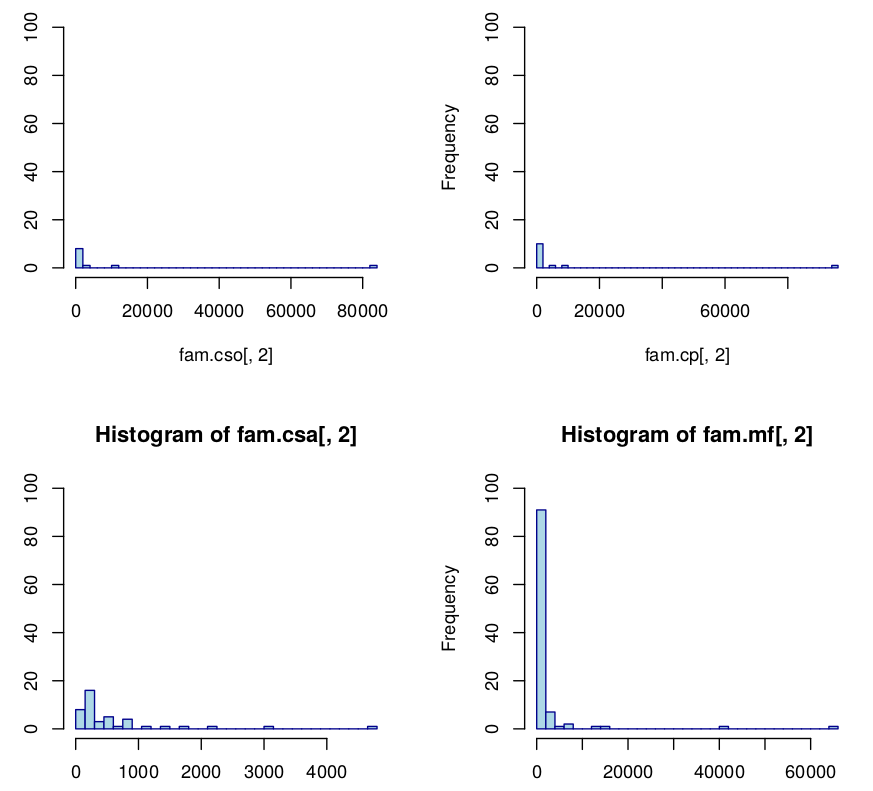
\includegraphics[scale=0.45]{img/distribution_familles.png}
			\caption{\textbf{Distribution des familles en fonction du nombre de séquences.}}
			\label{dist_fam} 
		\end{figure}
		
		\begin{figure}	
			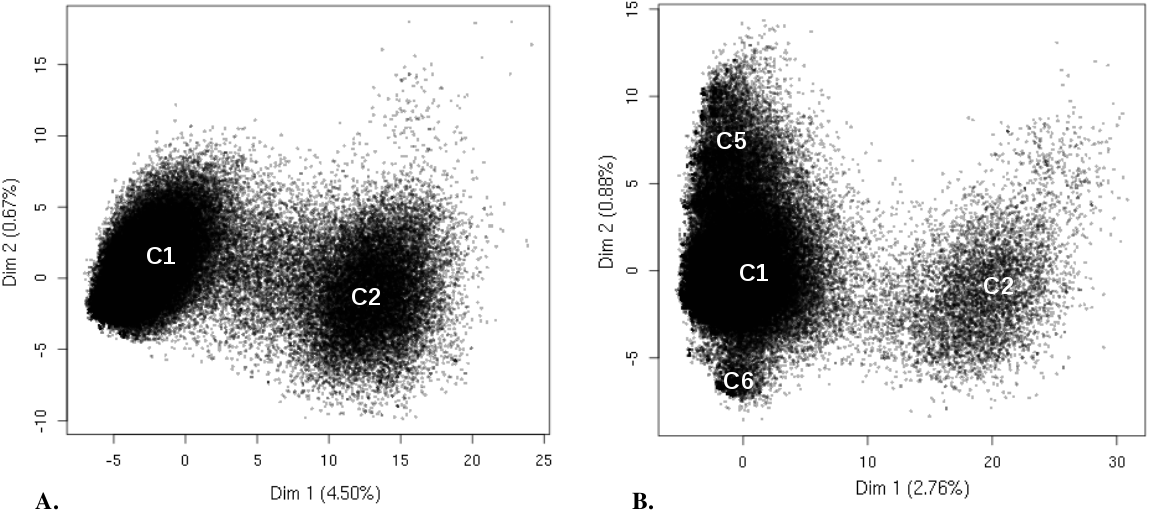
\includegraphics[scale=0.4]{img/ACP_experimental.png}  \\
			\caption{\textbf{Caractérisation visuelle des familles $\alpha$-satellite chez \textit{C. solatus} et \textit{C. pogonias} à partir d'une ACP, basée sur la composition en 5-mers des monomères :} Le nom des familles est indiqué sur les graphiques. Un point représente un monomère. \textbf{A.} \textit{C. solatus}. \textbf{B.} \textit{C. pogonias}.}
			\label{fig:ACP_exp} 
	\end{figure}
			

		\begin{table}
		\caption{\textbf{Comparaison des classifications automatiques avec celles publiées précédemment \cite{Cacheux2016}, \cite{Cacheux2018}.} Les familles marquées d'une étoile sont des familles < 100 séquences, non conservées pour la suite des analyses.}
			\center
			\begin{tabular}{|l|c|c|}
			\hline
			\textbf{Classes empiriques} & \multicolumn{2}{c|}{\textbf{Familles}} \\
	    	\hline
			\textbf{Classification publiée} &  \textbf{\textit{C. solatus}}  & \textbf{\textit{C. pogonias}}\\
			\hline
			C1 (> 5 000 séquences) &  1  & 9\\
			\hline
			C2 (> 82 000 séquences) & 10  & 2 \\
			\hline
			C3 (<170 séquences) & 1* & 1 \\
			\hline
			C4 (<170 séquences) & 1* & 1* \\
			\hline
			C5 (~ 8 300 séquences)& - 	 &  1 \\
			\hline
			C6 (~ 4 100 séquences) & -   &  0 \\
			\hline
			\end{tabular}
		\label{tab_count_fam}
	\end{table}
		
	Bien que le nombre de grandes familles soit relativement proche entre ces deux espèces (pour rappel 11 et 13), les résultats diffèrent significativement (Table \ref{tab_count_fam}). Chez \textit{C. solatus}, les classes C1 à C4 sont retrouvées: 11 familles correspondent à C2, une famille correspond à C1 et les familles C3 et C4, ne comportant que 109 et 112 séquences dans le jeu de données, sont retrouvées dans des petites familles d'environ 80 séquences chacune. Chez \textit{C. pogonias}, contrairement à C6, les classes C1, C2, C3, C4 et C5 sont retrouvées. C1 est répartie en 9 familles, alors que les classes C2, C3 et C5 sont regroupées dans des familles individuelles, et la classe C4 est également retrouvée sous la forme d'une petite famille de 86 séquences. La classe C2 chez le \textit{C. solatus} et la classe C1 chez \textit{C. pogonias} aurait dû former une famille chacune. Ces classes sont donc sur-clusterisées. Dans la suite de l'analyse, la pertinence de cette sur-clusterisation est examinée (plus particulièrement pour les séquences C2).
	
		\begin{figure}	
			\begin{tabular}{cc|cc}
				  & \textit{C. solatus} &  &  \textit{C. pogonias}\\
		\textbf{A} & 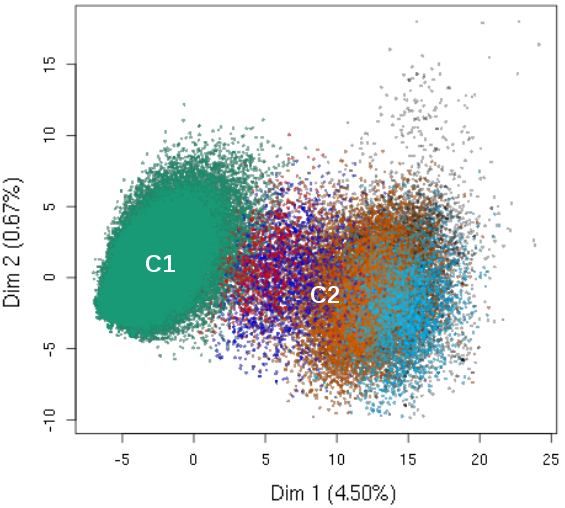
\includegraphics[scale=0.35]{img/solatus_ACP1.png} & \textbf{C} & 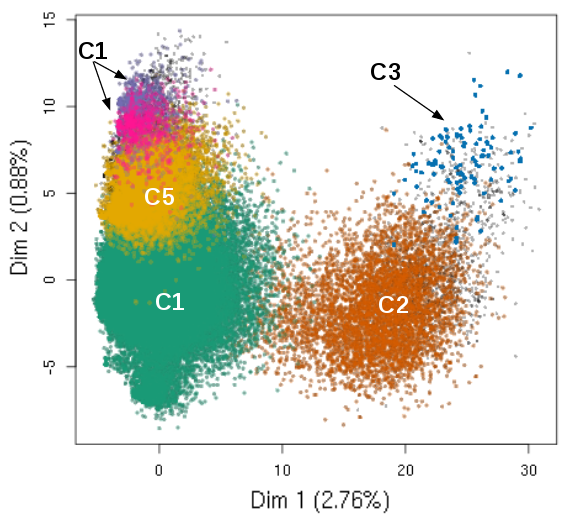
\includegraphics[scale=0.35]{img/pogonias_ACP1.png} \\
		\textbf{B} & 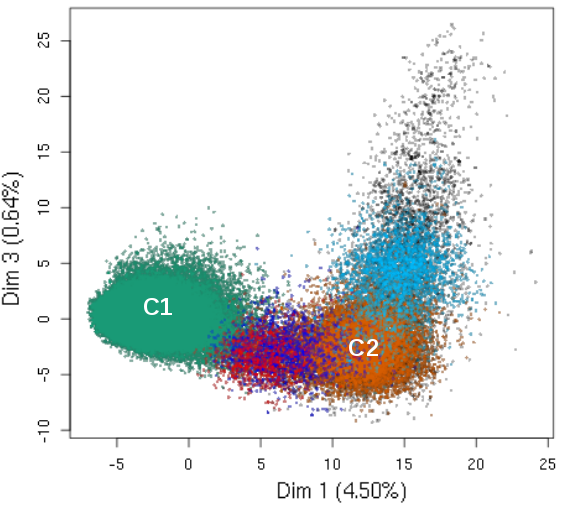
\includegraphics[scale=0.35]{img/solatus_ACP2.png} &  \textbf{D} & 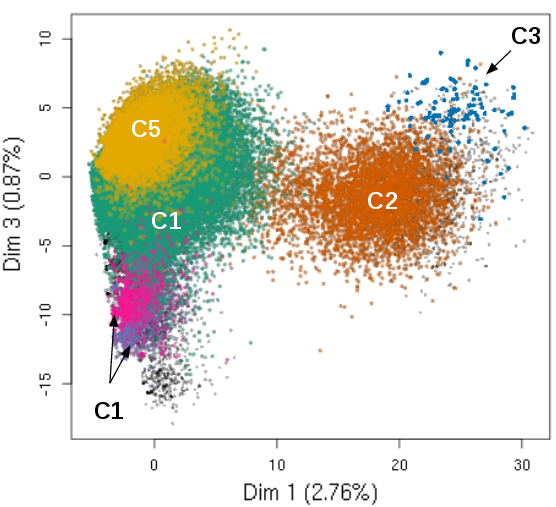
\includegraphics[scale=0.35]{img/pogonias_ACP2.png} \\
		\textbf{E} & 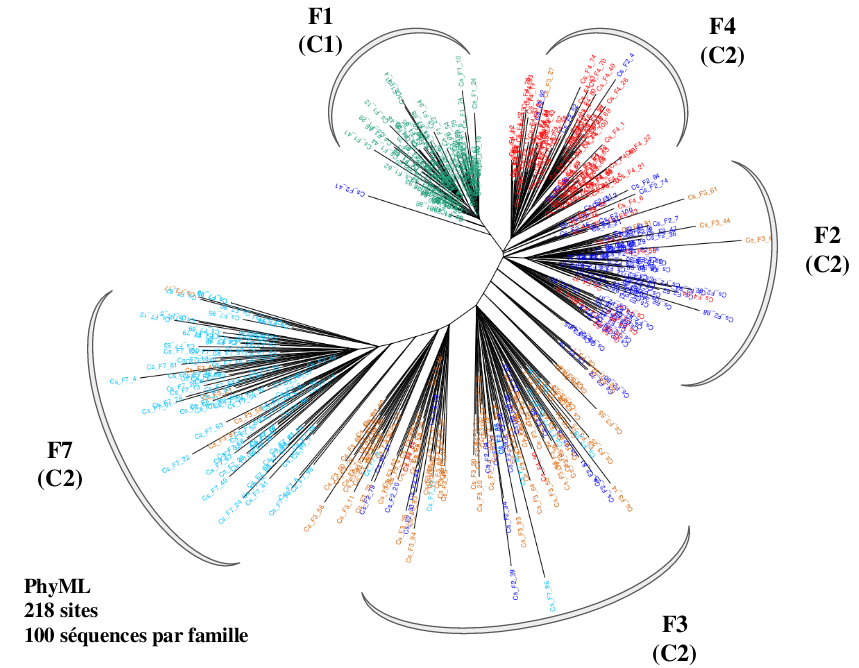
\includegraphics[scale=0.25]{img/tree_solatus.png} & \textbf{F} & 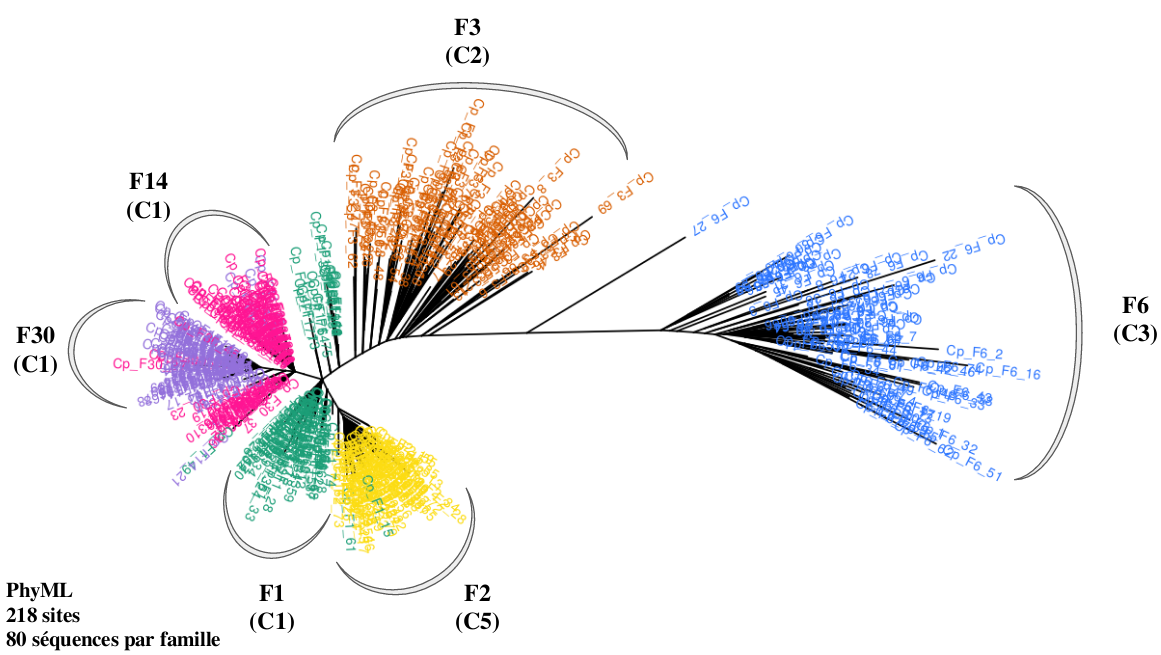
\includegraphics[scale=0.21]{img/tree_pogonias.png} \\
	\end{tabular}
	\caption{\textbf{Représentation des plus grandes familles issues de la classification automatisée:} Ces familles sont superposées sur les représentations de l'ACP des 5-mers.
	\textbf{A.} Composantes 1 et 2 de l'ACP. Les familles qui correspondraient à C1 sont en vert, C2 en orange, rouge, bleu et turquoise.  \textbf{B.} Composantes 1 et 3 de l'ACP. 
	\textbf{C.} Composantes 1 et 2 de l'ACP. Les familles qui correspondraient à C1 sont en vert, violet et rose, C2 en orange, C4 en bleu clair et C5 en jaune.
	\textbf{C.} Composantes 1 et 3 de l'ACP.
	\textbf{E. et F.} Phylogénie des différentes familles chez \textit{C. solatus} (100 séquences par famille) et \textit{C. pogonias} (80 séquences par famille) respectivement. Les couleurs sont respectivement conservées.	 
	\label{fig:so_po_acp_tree}
		} 
\end{figure}
			
			La diversité de ces classes a été analysée avec une ACP basée sur la composition en 5-mers des séquences (Figure \ref{fig:so_po_acp_tree}) afin de valider la sur-clusterisation observée. Les familles, représentées par une couleur, sont superposées sur les classes empiriques (en noir, non visible).
			
			  Chez \textit{C. solatus}, la classe C1 est entièrement retrouvée en une famille en vert. La classe C2 est répartie en 11 familles. Seules les 4 familles les plus grandes sont représentées par soucis de visibilité. Parmi celles-ci, deux familles intermédiaires (rouge et bleue) sont visibles entre la famille en vert  et  celle en orange. Elles se superposent.  Une famille supplémentaire turquoise se démarque. Pour confirmer cette division des séquences de C2, la visualisation de l'ACP des 5-mers est observée en fonction des composantes 1 et 3. Les familles intermédiaires sont toujours confondues, contrairement à la famille turquoise qui forme visuellement une famille à part entière. Pour confirmer cette classification, 50 séquences aléatoires par famille (représentée sur l'ACP) sont utilisées pour construire un arbre phylogénétique, et chacune des familles est représentée par une couleur. Chaque couleur se regroupe, donc l'arbre atteste que chaque famille est bien retrouvée, notamment les familles intermédiaires (rouge et bleue) qui forment bien deux familles. 
			  
			  Chez \textit{C. pogonias}, les classes C2, C3 et C5 sont bien retrouvées respectivement en orange, bleu foncé et jaune. La classe C6 n'est pas séparée de la classe C1 (en vert). La classe C1 est divisée en deux familles supplémentaires (en rose et violet). La visualisation des composantes 1 et 3 de l'ACP ne permet pas de trancher sur la l'individualité de ces deux familles. Pour cela, 50 séquences aléatoires par famille sont utilisées pour construire un arbre phylogénétique, et chacune des familles est représentée par une couleur. Chacune des couleurs se regroupe, justifiant la classification. Par ailleurs cet arbre montre que les familles en rose et violet sont très proches.
			
			En conclusion, la classification automatique permet de retrouver les classes identifiées dans les travaux publiés, exceptée la classe C6 qui semble indissociable de la classe C1, et la mise en évidence de plusieurs familles les classes C2 chez \textit{C. solatus} et C1 chez \textit{C. pogonias}.
			 
			\subsubsection{Motifs potentiellement fonctionnels}
\begin{figure}
	\center	
	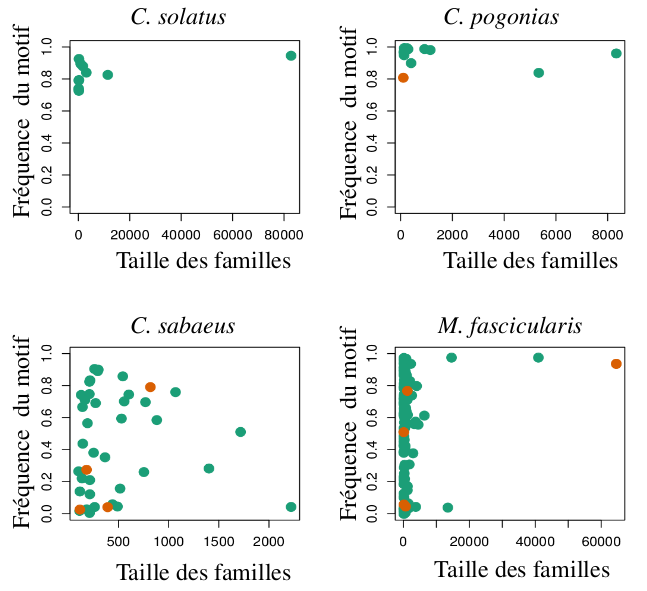
\includegraphics[scale=0.45]{img/graphique_motifs.png}
	\caption{\textbf{Fréquences des motifs CENP-B, pJ$\alpha$ ou pK$\beta$ dans les familles:} Les motifs ont été cherchés sur la base de leur consensus en autorisant deux différences. Le pourcentage de séquences par famille ayant le motif pJ$\alpha$ est en vert, pK$\beta$ en orange et CENP-B est absent de toutes les familles. Chaque famille est également représentée en fonction de sa taille.
	\label{fig:motif}} 
\end{figure}

			Ensuite je m'intéresse aux caractéristiques des familles $\alpha$-satellites identifiées, notamment l'existence de motifs conservés. A ce jour, les motifs CENP-B et pJ$\alpha$, capables de fixer respectivement les protéines CENP-B et pJ$\alpha$ (une protéine peu décrite), ont été décrits. Des travaux en cours dans l'équipe suggèrent l'existence d'un troisième motif conservé, nommé pK$\beta$, qui serait présent dans certaines familles. Ces trois motifs sont exclusifs l'un de l'autre. Ils sont situés au même endroit sur une séquence. Ils ont été recherchés pour chaque famille de chaque espèce sur la base de leur consensus, avec 2 \textit{mismatch} autorisés (cf matériel et méthodes).
			
			La protéine CENP-B est présente chez toutes les espèces de primates, mais les Cercopithèques ne possèdent pas son site de liaison. En effet, le motif CENP-B est absent chez \textit{C. solatus} et \textit{C. pogonias}. \textit{C. sabaeus} et \textit{M. fascicularis} n'ont pas ce motif non plus. Plus de 90\% des familles chez les quatre espèces ont le motif pJ$\alpha$ mais à des fréquences variables, et seulement 9\% ont le motif pK$\beta$ et quelques rares familles n'ont aucun des trois motifs chez \textit{M. fascicularis} (Figure \ref{fig:motif}). 
			
		La totalité des familles chez \textit{C. solatus} ont le motif  pJ$\alpha$ à plus de 72\%. Chez \textit{C. pogonias}, 12 familles sur 13 ont le motif à plus de 83\%. Une grande famille par espèce (> de 80 000 séquences), qui correspond à C1, a le motif à 95\%. \textit{C. sabaeus} présente 39 familles sur 43 avec ce motif, dont 7 l'ayant à plus de 75\%. \textit{M. fascicularis} a des pourcentages pour le motif pJ$\alpha$ qui varient entre 1\% et 97\%, dont 28 familles avec le motif à plus de 75\%.
		
			Une seule famille, incluant les séquences de C3, a ce motif à 80\% chez \textit{C. pogonias} et \textit{C. solatus} (non représenté car famille < 100 séquences). \textit{C. sabaeus} a quatre familles avec le motif, dont deux à 79\% et l'autre à 29\%. \textit{M. fascicularis} a cinq familles avec ce motif. La famille ayant le motif à 93\% est une grande famille de 64 000 séquences. Les deux autres familles ont le motif à 0.76\% et 0.50\%.
			
			Pour conclure sur les $\alpha$-satellites de ces espèces, le motif CENP-B est absent, le motif pJ$\alpha$ est le plus présent et le mieux conservé. Le motif pK$\beta$ est, quant à lui, présent dans très peu de familles.
				
			\subsubsection{Similarité entre familles}
\begin{figure}	
	\center
	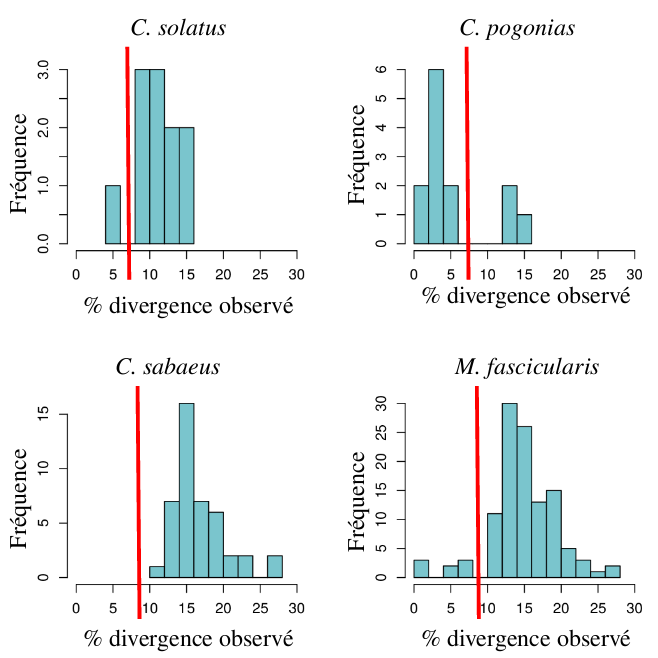
\includegraphics[scale=0.4]{img/hist_similarity.png}
	\caption{\textbf{Pourcentage de divergence observée dans les familles:} Histogramme du nombre de familles en fonction du pourcentage de divergence observé au sein de celles-ci. Un même seuil est observé chez chaque espèces et il est indiqué en rouge sur chaque histogramme. 
	\label{fig:divergence}
		} 
\end{figure}

	Selon les hypothèses actuelles \cite{Rudd2006}, les familles $\alpha$-satellites seraient le résultat d'amplifications qui généreraient plusieurs centaines ou milliers de copies identiques au cours du temps. La divergence intra-famille a été estimée à partir d'un échantillon de 500 séquences aléatoires par famille afin d'estimer l'âge des familles, les familles anciennes ayant un taux de divergence élevé. 
	
	Lorsque les histogrammes sont observés dans la globalité, un seuil à 8\% délimite le taux de divergence des familles. \textit{C. solatus} et \textit{C. pogonias} ont des pourcentages relativement faibles ne dépassant pas 15\%, le \textit{M. fascicularis} a des taux de divergence variant de 0.1\% à 28\%, et \textit{C. sabaeus} a les valeurs les plus élevées allant de 11\% à 28\% (Figure \ref{fig:divergence}).
	
	Chez \textit{C. solatus} et \textit{C. pogonias}, les familles qui ont un taux de divergence inférieur à 8\% correspondent à du C1 et C5 chez \textit{C. pogonias}. Les familles qui ont un taux de divergence supérieur correspondent à du C2, et pour \textit{C. pogonias} à C3 également. \textit{C. sabaeus} n'a que des familles avec un taux de divergence élevé, supérieur à 10\%. \textit{M. fascicularis} a quelques familles avec un faible pourcentage de divergence et d'autres à 30\%. 
	
	Pour conclure, une distribution bimodale est plus ou moins observée, avec des familles peu divergentes, notamment les familles qui correspondent à C1, et d'autres plus divergentes, notamment les familles qui correspondent à C2.
	
%%%%%%%%%%%%%%%%%%%%%%%%%%%%%%%%%%%%%%%%%%%%%%%%%%%%%%%%%%%%%%%%%
%%%%%%%%%%%%%%%%%%%%%%Résultats 2%%%%%%%%%%%%%%%%%%%%%%%%%%%%%%%%
%%%%%%%%%%%%%%%%%%%%%%%%%%%%%%%%%%%%%%%%%%%%%%%%%%%%%%%%%%%%%%%%% 
	\subsection{Comparaison inter-espèce}
	Pour comparer les classifications obtenues au sein de chaque espèce, une super-classification a été effectuée afin de déterminer l'existence de super-familles (SF). Pour cela, l'algorithme de classification a été utilisé sur un jeu de données composé de 100 séquences par grande famille (> 100 séquences) tirées aléatoirement pour chaque espèce. Un jeu de données de 18 100 séquences est ainsi créé à partir des 181 familles au total, puis soumis à la classification automatique. A l'issue de cette super-classification, 158 familles sont obtenues, dont 90 grandes familles (Figure \ref{distribution_SF}). Les petites familles de moins de 20 séquences, soit 1.76\% de ce jeu de données, ne sont pas prises en compte dans l'analyse. Après avoir présenté quelques caractéristiques de cette analyse, je présenterai les résultats concernant l'origine du site de fixation de pK$\beta$ et la divergence des séquences appartenant à C2.
	
	\begin{figure}	
	\center
	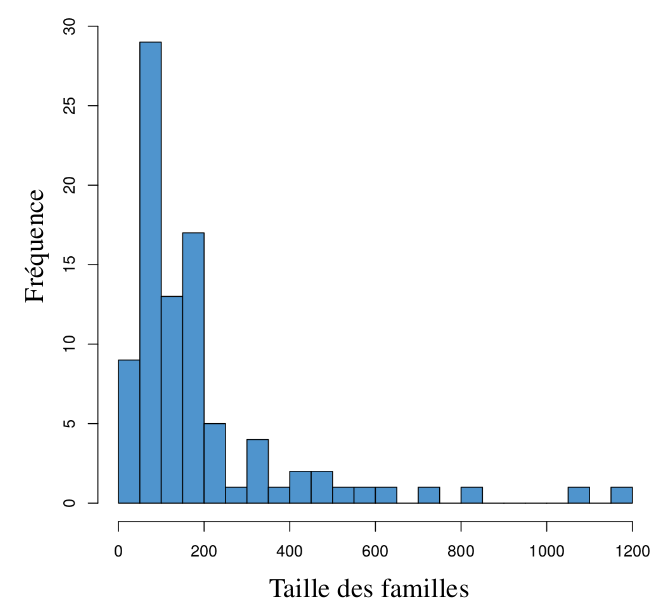
\includegraphics[scale=0.3]{img/distribution_SF.png}
	\caption{\textbf{Distribution des super-familles:} Histogramme du nombre de familles observées en fonction de la taille. 
	\label{distribution_SF}
		} 
	\end{figure}
	
	\subsubsection{Répartition des super-familles}
	Parmi les super-familles, seulement une \textit{a priori} est commune aux quatre espèces. Elle rassemble 6 familles parmi les 10 familles classées C2 de \textit{C. solatus} et les deux familles également classées C2 de \textit{C. pogonias}, ainsi que deux familles du \textit{M. fascicularis} et une famille du \textit{C. sabaeus}. La classe C2, du moins une partie, serait donc commune aux quatre espèces.
	
	Une super-famille est partagée entre  \textit{C. pogonias},  \textit{C. sabaeus} et  \textit{M. fascicularis}. Cette super-famille regroupe des familles ayant le motif pK$\beta$ uniquement et correspondrait à la classe C3 identifiée chez \textit{C. pogonias} et \textit{C. solatus}. Donc cette famille serait en fait commune aux 4 espèces également. Pour rappel, les séquences de la  classe C3 de \textit{C. solatus} n'ont pas été prises en compte à cause de la taille de la famille (< 100 séquences).
	
	Certaines super-familles sont spécifiques aux espèces. Au sein des 8 super-familles spécifiques de \textit{C. pogonias}, seule l'une d'entre elles regroupe deux familles, le reste étant composé d'une famille. Ces super-familles correspondraient à 5 familles C1, une famille C5 et une petite partie de C6. Les trois super-familles spécifiques de \textit{C. solatus} seraient équivalentes aux familles C2.  \textit{C. sabaeus} en aurait 3 et  \textit{M. fascicularis} 35.
	
	\textit{C. sabaeus} et \textit{M. fascicularis} partagent 38 super-familles, soit 42\% des grandes super-familles (> 20 séquences), dont la plus grande fait une taille de 1194 séquences. Une seule super-famille est uniquement commune à \textit{C. solatus} et \textit{C. pogonias} et elle regroupe les deux plus grandes familles qui correspondraient à du C1.
	
	\subsubsection{Un groupe C2 hétérogène}
			\begin{figure}
			\center	
			\begin{tabular}{cc}
 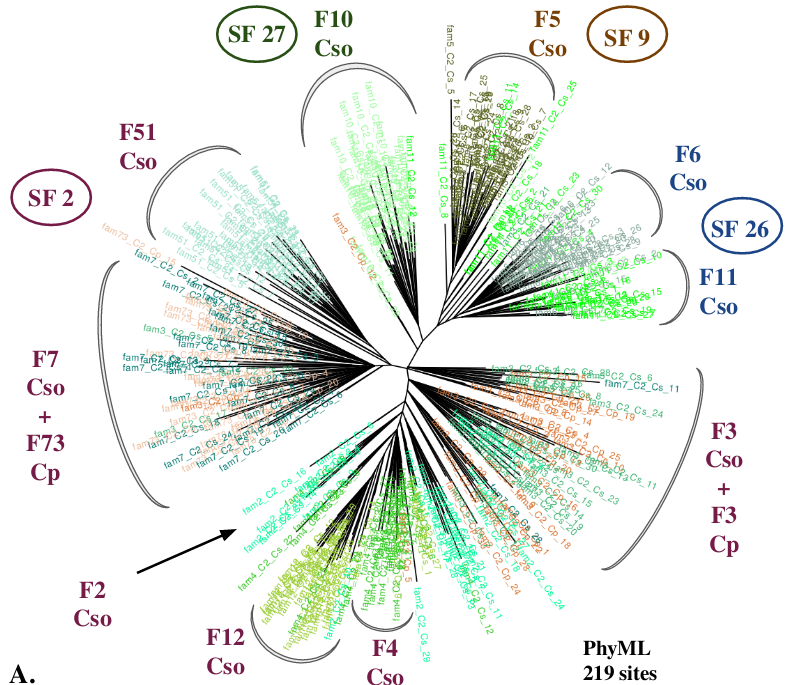
\includegraphics[scale=0.32]{img/tree_C2_pogonias_solatus.png}  & 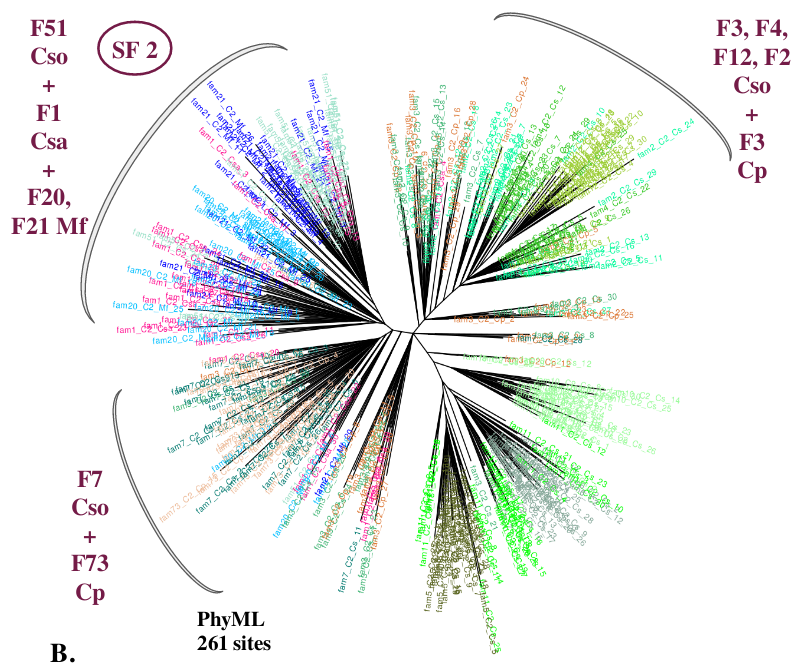
\includegraphics[scale=0.32]{img/tree_C2_all_species.png} \\
	\end{tabular}
	\caption{\textbf{Phylogénie des différentes familles qui correspondraient à la famille C2:}
	Les abbréviations: F = famille, SF = super-famille, Cso = \textit{C. solatus}, Cp = \textit{C. pogonias}, Mf = \textit{M. fascicularis}, Csa = \textit{C. sabaeus}. Les super-familles sont écrites d'une même couleur. \textbf{A.} \textit{C. solatus} (tons verts) et \textit{C. pogonias} (tons orange) \textbf{B.} Des familles du \textit{M. fascicularis} (tons bleus) et \textit{C. sabeus} (rose) sont rajoutées.	 
	\label{tree_C2}} 
\end{figure}

		La classe C2 est divisée en 10 familles chez \textit{C. solatus} et en 2 familles chez \textit{C. pogonias}. Or dans les résultats empiriques publiés, les séquences C2 auraient dû former une seule famille chez chacune de ces deux espèces. La classe C2 est donc sur-clusterisée. Ensuite, certaines de ces familles se sont regroupées pour former une super-famille, notamment avec une famille de \textit{C. sabaeus} et \textit{M. fascicularis}.
		
		Pour vérifier les résultats de cette super-classification, 30 séquences aléatoires de chacune des familles qui correspondraient à  C2 sont utilisées pour construire deux arbres phylogénétiques. Le premier contient uniquement les familles de \textit{C. solatus} représentées en tons verts et celles de \textit{C. pogonias} en tons orange (Figure \ref{tree_C2} A). Le second contient les familles supplémentaires supposées de la classe C2 de \textit{C. sabaeus} en rose et \textit{M. fascicularis} en tons bleus (Figure \ref{tree_C2} B).
		
		Dans le premier arbre (Figure \ref{tree_C2} A), chaque ton vert forme un groupe. Donc les familles de \textit{C. solatus} forment bien des familles distinctes. Seule une famille semble se mélanger aux autres. Deux de ces familles contiennent des tons orange. Donc \textit{C. solatus} et \textit{C. pogonias} partagent deux familles. Cette sur-clusterisation aurait donc du sens. Par contre, la super-famille regroupe trop de familles sans faire de distinction. Dans le second arbre (Figure \ref{tree_C2} B), les séquences du \textit{M. fascicularis} et \textit{C. sabaeus} vont spécifiquement se mettre avec une famille de \textit{C. solatus}.	

		Pour conclure sur l'hétérogénéité de  C2, une partie de ces familles est spécifique à \textit{C. solatus}, deux sont communes à \textit{C. solatus} et \textit{C. pogonias}, une famille de \textit{C. solatus} est commune aux quatre espèces selon la classification. Cependant la super-classification ne sépare pas aussi bien les familles.
						
	\subsubsection{Origine du motif pK$\beta$}
	
	\begin{figure}	
			\centering
				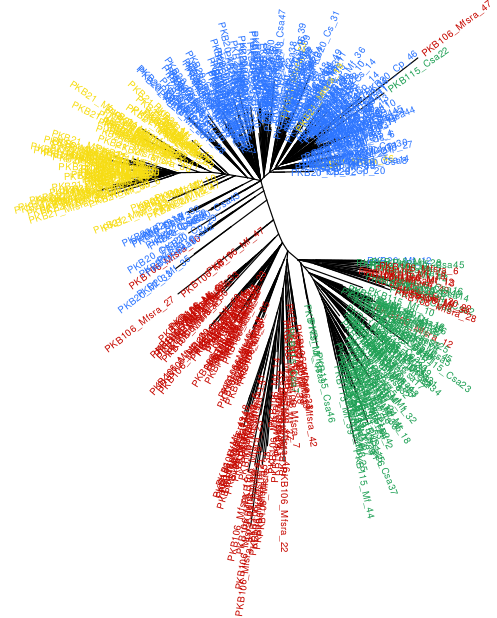
\includegraphics[scale=0.4]{img/pkb_tree.png}				
				\caption{\textbf{Phylogénie des super-familles pK$\beta$:} Les abbréviations: SF = super-famille, Cp = \textit{C. pogonias}, Cso = \textit{C. solatus}, Csa = \textit{C. sabaeus}, Mf = \textit{M. fascicularis}. Une couleur correspond à une super-famille. 
	\label{fig:pkb_tree}} 
	\end{figure}

	Pour poursuivre l'étude sur les familles communes entre espèces, le regroupement des familles $\alpha$-satellites ayant  le motif pK$\beta$ ou "familles pK$\beta$" attirent l'attention. 
	
	La première super-famille pK$\beta$ regroupe une famille de chacune des espèces. Ces familles pK$\beta$ possèdent le motif à 80\%. De plus cette famille correspond à la classe C3. Donc toutes ces espèces auraient une "famille C3" en commun. Le \textit{M. fascicularis} et \textit{C.sabeus} ont deux super-familles pK$\beta$ en commun. Les familles constituant ces super-familles ont un pourcentage de présence du motif relativement faible, pourtant elles sont tout de même rassemblées.  \textit{C.sabeus} et \textit{M. fascicularis} ont respectivement une et deux super-familles pK$\beta$ spécifiques. La première super-famille a le motif à 27\% et la deuxième à 50\%.
		
	Un arbre composé de toutes les familles pK$\beta$ est construit pour voir si les super-familles sont retrouvées phylogénétiquement. Le jeu de données est construit à partir de 50 séquences aléatoires par famille pK$\beta$ par espèce (Figure \ref{fig:pkb_tree}). Une couleur représente une super-famille. Chaque couleur se regroupe, donc les super-familles sont retrouvées. Les séquences se rassemblent exactement comme dans les super-familles.
	
	Pour conclure, les familles pK$\beta$ sont des familles partagées entre espèces pour certaines, et spécifique à une espèce pour d'autres. La méthode de classification retrouve bien les familles pK$\beta$ (intra-spécifique) et les super-familles pK$\beta$ inter-spécifique).

%%%%%%%%%%%%%%%%%%%%%%%%%%%%%%%%%%%%%%%%%%%%%%%%%%%%%%%%%%%%%%%%%%
%%%%%%%%%%%%%%%%%%%%%%%%Discussion%%%%%%%%%%%%%%%%%%%%%%%%%%%%%%%%
%%%%%%%%%%%%%%%%%%%%%%%%%%%%%%%%%%%%%%%%%%%%%%%%%%%%%%%%%%%%%%%%%%
\section{Discussion}

	Après classification, les séquences $\alpha$-satellites sont réparties en familles. Le nombre de familles par espèce est très variable. \textit{C. solatus} et \textit{C. pogonias} ont seulement un dizaine de familles comparé au \textit{M. fascicularis} qui en a un peu plus d'une centaine. \textit{C. sabaeus} a un nombre intermédiaire de famille.

	La méthode de classification crée beaucoup de petites familles (< 100 séquences). Par conséquent, plusieurs séquences sont éliminées et celles-ci pourraient être  une famille caractéristique. Ces familles de petite taille sont probablement des séquences ayant subi des réarrangements, ayant une délétion importante, ou dont la qualité est moins bonne. De plus très peu d'information est perdue.

	Bien que la méthode de classification ait retrouvé la majorité des familles empiriques, elle n'a pas réussi à dissocier les séquences C6 de C1. Par contre, elle a pu diviser C1 chez \textit{C. pogonias} et C2  chez \textit{C. solatus}. Cet algorithme de classification a du mal à séparer des séquences qui se seraient trop proches mais il peut séparer un groupe qui n'est pas parfaitement homogène. En effet les divisions du groupe C2 ont bien été retrouvées sur un arbre phylogénétique pour \textit{C. solatus}.

	La fonction la mieux conservée est celle derrière le motif pJ$\alpha$. Il est présent dans pratiquement toutes les familles, même si sa présence est moindre dans quelques une des familles chez \textit{C. sabeus} et \textit{M. fascicularis}. La fonction de pK$\beta$, bien que largement moins présente, reste très conservée. De plus, certaines super-familles sont communes à plusieurs espèces. Parmi celles-ci, les plus anciennes sont la super-famille spécifique à \textit{C. sabaeus} et celle spécifique au \textit{M. fascicularis}, avec un pourcentage de divergence de 17,50\% et 16,12\% respectivement. La famille la plus jeune est la deuxième super-famille spécifique au macaque avec 7,09\% de divergence.  La super-famille commune aux 4 espèces est relativement ancienne, avec en moyenne 14,70\% de divergence, et les familles communes à la fois au \textit{M. fascicularis} et au \textit{C. sabaeus} sont un peu plus jeune avec respectivement 12,50\% et 11.80\% de divergence.

	Chez \textit{C. solatus} et \textit{C. pogonias}, les séquences C1 ont le pourcentage de divergence le plus faible, elles sont donc des familles jeunes. Les séquences de la famille C2, et C3 chez \textit{C. poginias}, ont les pourcentages de divergence les plus élevés. Ce sont les familles les plus anciennes.  La distribution bimodale pourrait supposer des vagues d'amplification.

	La méthode de classification, confirmée par l'analyse phylogénétique, rassemble une famille de \textit{C. sabaeus} et deux familles du \textit{M. fascicularis} avec des séquences C2 de \textit{C. solatus} et \textit{C. pogonias}. Ces espèces ont donc des séquences qui seraient potentiellement des séquences C2. Les taux de divergence relativement élevés, autour de 14\% pour ces familles, s'accorde avec cette information. Cependant il pourrait y avoir d'autres séquences de C2 qui ne seraient pas détectées. Certaines de ces séquences forment une super-famille commune aux 4 espèces tandis que d'autres sont spécifiques à une seule espèce. Ces informations permettent de déduire l'ordre d'apparition des familles. La super-famille C2 commune aux 4 espèces serait une famille ancienne qui serait apparue bien avant les autres. Les familles un peu plus récentes seraient celles partagées entre \textit{M. fascicularis} et \textit{C. sabaeus}, et celles qui sont spécifiques aux espèces seraient les plus récentes. Bien que le \textit{C. sabaeus} soit plus proche des cercipithèques, il partage plus de familles avec \textit{M. fascicularis}. Il est possible que certaines familles de \textit{C. solatus} et \textit{C. pogonias} ne figurent pas parmi les résultats, car toutes les familles n'ont pas été détectées par l'enzyme de restriction. 

	Pour évaluer la reproductibilité,  plusieurs super-classifications ont été lancées et analysées. Avec les mêmes paramètres, d'une super-classification à l'autre, les super-familles obtenues sont différentes. Seules les familles pK$\beta$ se rassemblent exactement de la même manière. Des séquences C2 sont regroupées, mais pas de la même manière. Elles peuvent former une seule famille et parfois plusieurs familles. Cette méthode de classification possède donc un problème de reproductibilité.  
	
\section{Conclusion}
	Pour conclure, les séquences  $\alpha$-satellites ont été réparties en familles, caractérisée en fonction de ce qui a été trouvé dans la littérature et en par la fonction des motifs caractéristiques, ainsi que par le pourcentage de similarité.  La super-classification a permis de trouver les familles communes entre espèces et de déduire les familles les plus anciennes et les plus récentes ou encore celles qui sont spécifiques.
	
	Il serait intéressant d'étudier la structure en HOR ou en organisation monomérique. Si les familles sont définies en une structure particulière, la question se pose de savoir si elles conservent la même structure d'une espèce à l'autre.

%%%%%%%%%%%%%%%%%%%%%%%%%%%%%%%%%%%%%%%%%%%%%%%%%%%%%%%%%%%%%%%%%%
%%%%%%%%%%%%%%%%%%%%%%%%Bibliographie%%%%%%%%%%%%%%%%%%%%%%%%%%%%
%%%%%%%%%%%%%%%%%%%%%%%%%%%%%%%%%%%%%%%%%%%%%%%%%%%%%%%%%%%%%%%%%
\newpage
\strut  ~  \mbox{}  \null
\newpage
\bibliographystyle{unsrt}
\bibliography{biblio}

%%%%%%%%%%%%%%%%%%%%%%%%%%%%%%%%%%%%%%%%%%%%%%%%%%%%%%%%%%%%%%%%%%
%%%%%%%%%%%%%%%%%%%%Résumé & Abstract%%%%%%%%%%%%%%%%%%%%%%%%%%%%%
%%%%%%%%%%%%%%%%%%%%%%%%%%%%%%%%%%%%%%%%%%%%%%%%%%%%%%%%%%%%%%%%%%
\newpage 
\thispagestyle{empty}
\section*{Résumé}~\\[0.2cm]
Chez les primates, des séquences centromériques répétées en tandem sont appelées ADN $\alpha$-satellite. Un monomère $\alpha$-satellite fait 171 pb de long. Elles ont un taux d'identité de 60\% à 100\%. Ces monomères peuvent être regroupés en familles selon la similarité. Pour étudier ces familles, des méthodes utilisant la phylogénie existent mais elles ne permettent pas de classer un grand nombre de séquences. De plus les méthodes ne sont pas objectives et ne permettent pas de comparer les espèces entre elles. Pour pallier ce problème,l'équipe ARChE a développé une méthode de classification permettant de traiter des centaines de milliers de séquences (2017). Mon sujet consiste à appliquer cette méthode aux jeux de données déjà publiés pour évaluer la méthode. Dans un deuxième temps, cette méthode est appliquée à deux autres primates dans le but de  caractériser les familles d'espèces proches. Les mécanismes d'évolution sont déduits à partir d'une comparaison inter-espèce révélant les différences et les familles communes. 

\section*{Abstract}~\\[0.2cm]
Centromeric repeated sequences in Primates are named $\alpha$-satellite DNA. An $\alpha$-satellite's length is about 171 pb. Its identity rate is between 60\% and 100\%. Monomers can be gathered into families according to their similarity. To study these families, methods using phylogeny are used but a large number of sequences cannot be processed. Moreover these methods are not objective and do not allow inter-species comparison.To overcome this problem, the team ARChE developped a classification method which processes hundred of thousands of sequences (2017). The subject of my internship is to apply this method to published datasets and assess this method. Then this method is applied to other Primates in order to caracterize families in close species. Mechanism of evolution are deducted from inter-specices comparison, revealing common and different families. 

%%%%%%%%%%%%%%%%%%%%%%%%%%%%%%%%%%%%%%%%%%%%%%%%%%%%%%%%%%%%%%%%%%
%%%%%%%%%%%%%%%%%%%%%%%%Annexes%%%%%%%%%%%%%%%%%%%%%%%%%%%%
%%%%%%%%%%%%%%%%%%%%%%%%%%%%%%%%%%%%%%%%%%%%%%%%%%%%%%%%%%%%%%%%%
\newpage
\thispagestyle{empty}
\begin{appendix}
\section*{Annexes}~\\[0.2cm]
    \begin{center}
        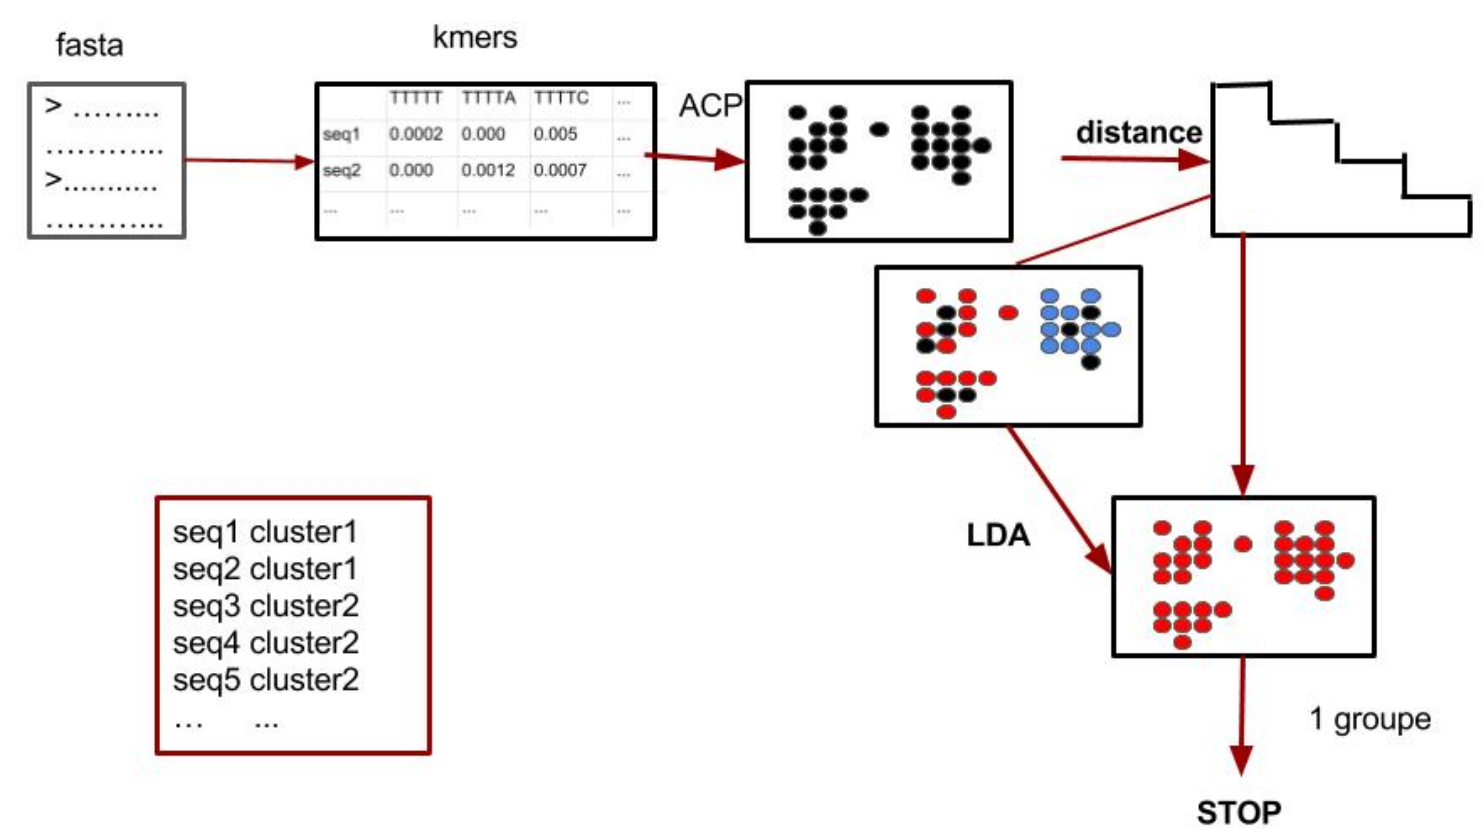
\includegraphics[scale=0.35, angle=0]{img/algo_classification.png}
        \label{a_micro}
    \end{center}
\end{appendix}

\end{document}
